\documentclass{ctsol}
\usepackage{tikz}

\title{ACM 算法与微应用实验室 2022 年 4 月月赛题解}
\date{2022 年 5 月 1 日}

\begin{document}

\maketitle
\addsolution{FMVP}{AgOH}{排序}
\addsolution{最强阵容}{AgOH}{分数规划}
\addsolution{八保舟}{AgOH}{莫队 + 值域线段树}
\addsolution{自古红蓝}{AgOH}{动态规划 + 矩阵加速}
\addsolution{5Yqg5a+G6YCa5L+h}{AgOH}{分层图最短路}
\addsolution{K-prime seive 2}{Tifa}{线性筛}

\section*{题目概览}

\solutiontab

\section*{鸣谢}

感谢 \href{https://github.com/Tiphereth-A}{\@Tifa} 大佬参与本次比赛的出题工作。

\makesolution
\section*{做法}

签到题

\section*{标程}

\std{A}

\makesolution
\section*{做法}

本题这种类型的题目叫做分数规划,通解是二分答案

发现题目要求即:在所有 $(a_i,b_i)$ 中选出 $5$ 对:$(a_j,b_j)$,使得 $\cfrac{\sum_{i=j}^{5}a_j}{\sum_{i=j}^{5}b_j}$ 最大

我们发现最大值这个东西是有单调性的,显然可以二分答案,而二分答案的关键在于 \verb|check| 函数的实现,设我们要判断的二分值为 $m$,则有:

$$
    \begin{aligned}
                    & \cfrac{\sum_{i=j}^{5}a_j}{\sum_{i=j}^{5}b_j} > m \\
        \Rightarrow & \sum_{i=j}^{5}a_j - m\sum_{i=j}^{5}b_j > 0 \\
        \Rightarrow & \sum_{i=j}^{5}a_j-mb_j > 0
    \end{aligned}
$$

也就是说只要我们能在所有 $(a_i,b_i)$ 中选出 $5$ 个 $(a_j,b_j)$ 使得 $\sum_{i=j}^{5}a_j-mb_j > 0$,那么我们的二分值 $m$ 就是满足条件的

二分实数答案要注意精度问题(eps)

\section*{标程}

\std{B}

\makesolution
\section*{做法}

容易发现,对于一个区间 $[l,r]$ 来说,能获得的最大总快乐值一定是贪心地先吃最大快乐值的冰淇淋,直到没有冰淇淋或剩余的冰淇淋的快乐值都为 $0$ 为止

因为所有冰淇淋一起减 $1$,相当于没减,所以一定要抢吃最大快乐值的冰淇淋

那么可以发现,快乐值小于区间长度一半的冰淇淋必然不会对最大总快乐值产生贡献,因为该吃它们的时候快乐值已经扣没了

于是对于整个区间内的冰淇淋来说,能获得的最大总快乐值为 $s-\cfrac{c(c-1)}{2}$,其中 $s$ 为快乐值大于区间长度一半的快乐值的总和,$c$ 为快乐值大于区间长度一半的快乐值的数量

值域不大只有 ${10}^5$,可以考虑使用值域线段树维护

\section*{标程}

\std{C}

\makesolution
\section*{做法}

方案数,又不像是组合数学,考虑动态规划

若最后一个格子未涂色,则倒数第二个格子可涂可不涂;若最后一个格子涂色了,则倒数第二个格子一定不能涂色,于是:

\begin{itemize}
    \item 状态设计:$dp[i]$ 代表已考虑了前 $i$ 个格子的方案数
    \item 初始状态:$dp[1] = 2,~dp[2] = 3$
    \item 转移方程:$dp[i] = dp[i-1] + dp[i-2]$
    \item 所求结果:$dp[n]$
\end{itemize}

即斐波那契数列,注意到 $n \leq {10}^{18}$ 很大,需要使用矩阵加速

\section*{标程}

\std{D}

\makesolution
\section*{做法}

设所给图为 $G_0=(V_0,E_0)$,将其复制 $k$ 份,分别记为 $G_1=(V_1,E_1),G_2=(V_2,E_2),\cdots,G_k=(V_k,E_k)$

设图 $G_i$ 中所有结点为 $u_{i,1},u_{i,2},\cdots,u_{i,m}$,对于所有结点 $u_{i,j} \in G_i~(i \neq k)$,连边:

$$u_{i,j} \xrightarrow{0} u_{i+1,t}~(u_{i,j} \rightarrow u_{i,t} \in E_i)$$

然后从 $u_{0,1}$ 结点开始跑一遍单源最短路径,答案即为:

$$\min\limits_{i=0}^{k}dis[u_{i,n}]$$

当然也可以用边把 $u_{0,n},u_{1,n},\cdots,u_{k,n}$ 这几个结点用边权为 $0$ 的边连接起来,然后答案即为 $dis[u_{k,n}]$

举个例子,第一个样例连边后所形成的图为:

\begin{center}
    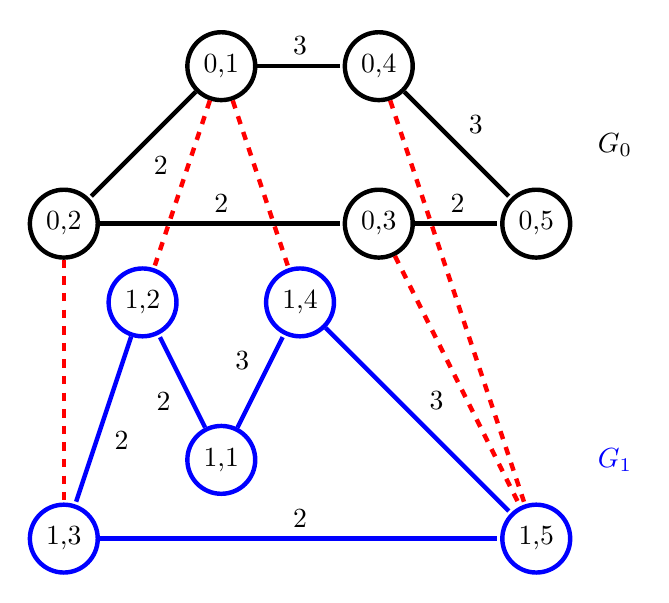
\begin{tikzpicture}
    [
        shorten >=1pt, auto, node distance=3cm, ultra thick,
        node0_style/.style={circle,draw=black},
        edge0_style/.style={draw=black, ultra thick},
        node1_style/.style={circle,draw=blue},
        edge1_style/.style={draw=blue, ultra thick},
        edgec_style/.style={draw=red, ultra thick, dashed}
    ]
        \node[node0_style] (v01) at (1,6) {0,1};
        \node[node0_style] (v02) at (-1,4) {0,2};
        \node[node0_style] (v03) at (3,4) {0,3};
        \node[node0_style] (v04) at (3,6) {0,4};
        \node[node0_style] (v05) at (5,4) {0,5};
        \draw[edge0_style] (v01) edge node{2} (v02);
        \draw[edge0_style] (v02) edge node{2} (v03);
        \draw[edge0_style] (v01) edge node{3} (v04);
        \draw[edge0_style] (v04) edge node{3} (v05);
        \draw[edge0_style] (v03) edge node{2} (v05);
    
        \node[node1_style] (v11) at (1,1) {1,1};
        \node[node1_style] (v12) at (0,3) {1,2};
        \node[node1_style] (v13) at (-1,0) {1,3};
        \node[node1_style] (v14) at (2,3) {1,4};
        \node[node1_style] (v15) at (5,0) {1,5};
        \draw[edge1_style] (v11) edge node{2} (v12);
        \draw[edge1_style] (v12) edge node{2} (v13);
        \draw[edge1_style] (v11) edge node{3} (v14);
        \draw[edge1_style] (v14) edge node{3} (v15);
        \draw[edge1_style] (v13) edge node{2} (v15);
    
        \draw[edgec_style] (v01) -- (v12);
        \draw[edgec_style] (v02) -- (v13);
        \draw[edgec_style] (v01) -- (v14);
        \draw[edgec_style] (v04) -- (v15);
        \draw[edgec_style] (v03) -- (v15);
    
        \node[text=black] at (6,5) {$G_0$};
        \node[text=blue] at (6,1) {$G_1$};
    \end{tikzpicture}
\end{center}

从结点 $u_{0,1}$ 开始跑一遍单源最短路径,可以发现 $dis[u_{0,n}]=6,dis[u_{1,n}]=3$,故答案为:

$$\min(dis[u_{0,n}],dis[u_{1,n}])=3$$

这种拆点后跑最短路的方法叫做分层图最短路

\clearpage
\section*{标程}

\std{E}

\makesolution
\section*{做法}

\section*{标程}

\std{F}

\end{document}
